\hypertarget{node-red-como-interface-supervisuxf3ria}{%
\chapter{Node-RED como Interface Supervisória}\label{node-red-como-interface-supervisuxf3ria}}

\section*{Objetivos de Aprendizagem}

Ao final deste capítulo, o leitor será capaz de:

\begin{itemize}
\tightlist
\item
  Descrever a arquitetura e os conceitos fundamentais do Node-RED.
\item
  Criar flows para aquisição de dados via Modbus TCP e MQTT.
\item
  Desenvolver dashboards de supervisão com o módulo node-red-dashboard.
\item
  Avaliar quando Node-RED é adequado como solução supervisória e suas limitações.
\end{itemize}

\begin{center}\rule{0.5\linewidth}{0.5pt}\end{center}

\hypertarget{o-que-uxe9-node-red}{%
\section{O que é Node-RED?}\label{o-que-uxe9-node-red}}

O \textbf{Node-RED} é uma plataforma de programação visual \emph{flow-based} desenvolvida pela IBM em 2013, inicialmente para conectar dispositivos de hardware, APIs e serviços online de forma rápida. Tornou-se open-source e hoje é mantido pela \textbf{OpenJS Foundation}.

Sua filosofia: \textbf{``wiring together''} --- conectar entradas, processamentos e saídas arrastando e soltando nós (\emph{nodes}) em um editor visual, sem escrever código complexo.

\textbf{Por que Node-RED para automação?}

\begin{itemize}
\tightlist
\item
  \textbf{Baixo custo:} open-source, sem licenciamento.
\item
  \textbf{Prototipagem rápida:} um flow funcional em minutos.
\item
  \textbf{Biblioteca ampla:} mais de 4.000 nodes na comunidade (Modbus, OPC UA, MQTT, HTTP, banco de dados).
\item
  \textbf{Leve:} roda em Raspberry Pi, gateways industriais, servidores Linux.
\item
  \textbf{Dashboard integrado:} módulo \passthrough{\lstinline!node-red-dashboard!} gera interfaces web sem HTML/CSS.
\end{itemize}

Na prática, o Node-RED costuma ocupar a posição de \textbf{camada de integração}: ele conversa com
quem tem protocolo industrial, normaliza e entrega para quem consome dado.

\begin{center}
\IfFileExists{../figuras/capitulo-07-m1.pdf}{%
  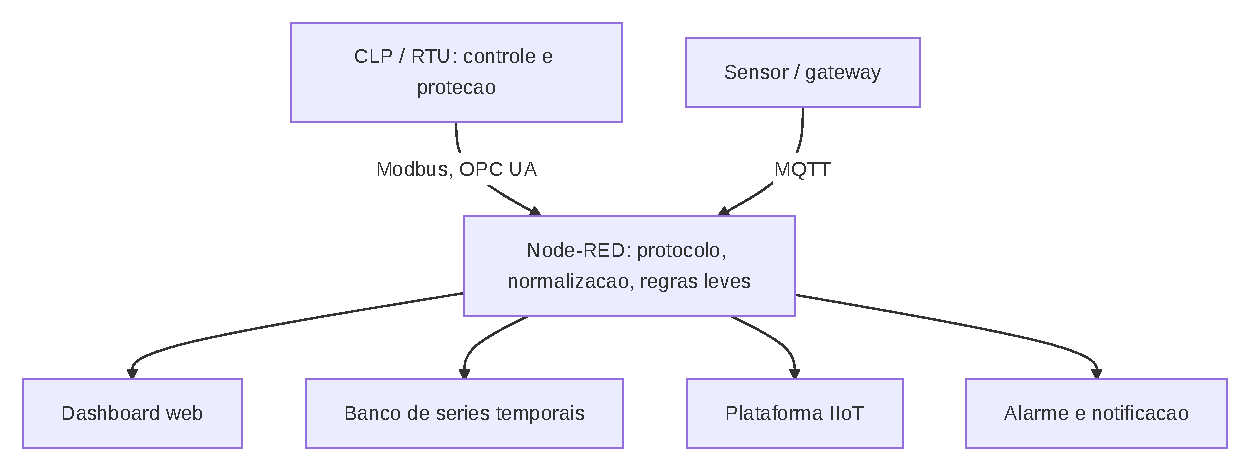
\includegraphics[width=\linewidth,height=0.8\textheight,keepaspectratio]{../figuras/capitulo-07-m1.pdf}%
}{\fbox{\parbox{0.9\linewidth}{\small Diagrama Mermaid ainda não renderizado: capitulo-07-m1. Rode scripts/render-mermaid.sh.}}}
\end{center}

\begin{figure}
\centering
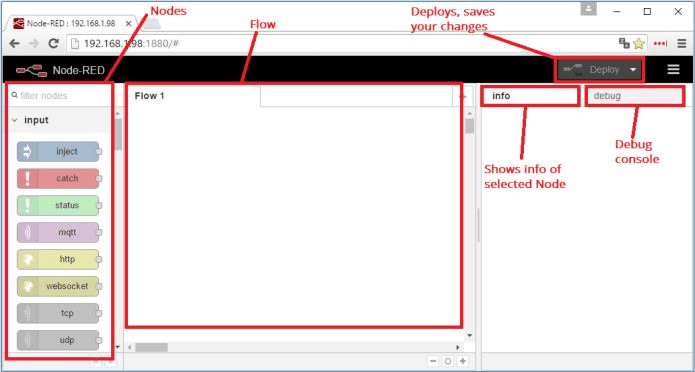
\includegraphics{../figuras/cap07-editor-node-red.png}
\caption[Figura 7.1 -- Interface do editor Node-RED]{Figura 7.1 -- Interface do editor Node-RED. \textbf{Fonte:} \emph{Node-RED --- Interface de Supervisão} (material do curso), p.~13.}
\end{figure}

O editor é uma única página web dividida em quatro regiões, cada uma com um papel definido:

\begin{longtable}[]{@{}
  >{\raggedright\arraybackslash}p{(\columnwidth - 4\tabcolsep) * \real{0.3333}}
  >{\raggedright\arraybackslash}p{(\columnwidth - 4\tabcolsep) * \real{0.3333}}
  >{\raggedright\arraybackslash}p{(\columnwidth - 4\tabcolsep) * \real{0.3333}}@{}}
\toprule\noalign{}
\begin{minipage}[b]{\linewidth}\raggedright
Região
\end{minipage} & \begin{minipage}[b]{\linewidth}\raggedright
Posição
\end{minipage} & \begin{minipage}[b]{\linewidth}\raggedright
Função
\end{minipage} \\
\midrule\noalign{}
\endhead
\bottomrule\noalign{}
\endlastfoot
\textbf{Palette} & esquerda & Catálogo de nodes disponíveis, agrupados por categoria \\
\textbf{Canvas} & centro & Área de desenho do flow; os fios ligam a saída de um node à entrada de outro \\
\textbf{Sidebar} & direita & Saída do node \passthrough{\lstinline!debug!}, ajuda do node selecionado, contexto e configurações \\
\textbf{Deploy} & topo & Publica o flow em edição para execução \\
\end{longtable}

A figura anota as três primeiras regiões. O botão \textbf{Deploy} é o que separa ``desenho'' de
``sistema em operação'': enquanto não for acionado, o processo continua rodando com a versão
anterior do flow.

\begin{center}\rule{0.5\linewidth}{0.5pt}\end{center}

\hypertarget{instalauxe7uxe3o-e-configurauxe7uxe3o}{%
\section{Instalação e Configuração}\label{instalauxe7uxe3o-e-configurauxe7uxe3o}}

\hypertarget{instalauxe7uxe3o-via-npm-linux-raspberry-pi}{%
\subsection{Instalação via npm (Linux / Raspberry Pi)}\label{instalauxe7uxe3o-via-npm-linux-raspberry-pi}}

\begin{lstlisting}[language=bash]
# Instalar Node.js (versão LTS recomendada)
curl -fsSL https://deb.nodesource.com/setup_18.x | sudo bash -
sudo apt-get install -y nodejs

# Instalar Node-RED globalmente
sudo npm install -g --unsafe-perm node-red

# Iniciar Node-RED
node-red
\end{lstlisting}

\hypertarget{instalauxe7uxe3o-via-docker}{%
\subsection{Instalação via Docker}\label{instalauxe7uxe3o-via-docker}}

\begin{lstlisting}[language=bash]
docker run -it -p 1880:1880 \
  -v node_red_data:/data \
  --name mynodered nodered/node-red
\end{lstlisting}

\hypertarget{acessando-o-editor}{%
\subsection{Acessando o Editor}\label{acessando-o-editor}}

Abra o navegador em: \passthrough{\lstinline!http://localhost:1880!}

\begin{caixadica}

\textbf{Dica:} Para uso em produção, configure o Node-RED com autenticação de usuários (arquivo \passthrough{\lstinline!settings.js!}), HTTPS e uma solução de inicialização automática como \passthrough{\lstinline!pm2!} ou \passthrough{\lstinline!systemd!}, para que o serviço reinicie automaticamente após reboot.

\end{caixadica}

\begin{center}\rule{0.5\linewidth}{0.5pt}\end{center}

\hypertarget{conceitos-fundamentais}{%
\section{Conceitos Fundamentais}\label{conceitos-fundamentais}}

\hypertarget{nodes-nuxf3s}{%
\subsection{Nodes (Nós)}\label{nodes-nuxf3s}}

Os \textbf{nodes} são os blocos de construção do Node-RED. Cada node realiza uma função específica:

\begin{longtable}[]{@{}
  >{\raggedright\arraybackslash}p{(\columnwidth - 4\tabcolsep) * \real{0.3333}}
  >{\raggedright\arraybackslash}p{(\columnwidth - 4\tabcolsep) * \real{0.3333}}
  >{\raggedright\arraybackslash}p{(\columnwidth - 4\tabcolsep) * \real{0.3333}}@{}}
\toprule\noalign{}
\begin{minipage}[b]{\linewidth}\raggedright
Categoria
\end{minipage} & \begin{minipage}[b]{\linewidth}\raggedright
Exemplos de Nodes
\end{minipage} & \begin{minipage}[b]{\linewidth}\raggedright
Função
\end{minipage} \\
\midrule\noalign{}
\endhead
\bottomrule\noalign{}
\endlastfoot
\textbf{Entrada (Input)} & \passthrough{\lstinline!mqtt in!}, \passthrough{\lstinline!modbus-read!}, \passthrough{\lstinline!http in!}, \passthrough{\lstinline!inject!} & Recebe dados ou eventos \\
\textbf{Processamento} & \passthrough{\lstinline!function!}, \passthrough{\lstinline!change!}, \passthrough{\lstinline!filter!}, \passthrough{\lstinline!json!} & Transforma ou filtra dados \\
\textbf{Saída (Output)} & \passthrough{\lstinline!mqtt out!}, \passthrough{\lstinline!modbus-write!}, \passthrough{\lstinline!http request!}, \passthrough{\lstinline!debug!} & Envia dados ou executa ações \\
\textbf{Dashboard} & \passthrough{\lstinline!gauge!}, \passthrough{\lstinline!chart!}, \passthrough{\lstinline!text!}, \passthrough{\lstinline!button!}, \passthrough{\lstinline!slider!} & Exibe dados na interface web \\
\textbf{Banco de Dados} & \passthrough{\lstinline!influxdb in!}, \passthrough{\lstinline!influxdb out!}, \passthrough{\lstinline!mongodb!} & Persistência de dados \\
\textbf{Utilitários} & \passthrough{\lstinline!delay!}, \passthrough{\lstinline!trigger!}, \passthrough{\lstinline!rbe!} (report-by-exception) & Controle de fluxo \\
\end{longtable}

\hypertarget{flows-e-wires}{%
\subsection{Flows e Wires}\label{flows-e-wires}}

Um \textbf{flow} é uma sequência de nodes conectados por \textbf{wires} (fios). Cada wire transporta uma mensagem (\passthrough{\lstinline!msg!}) do node anterior para o próximo.

A mensagem é um objeto JSON com campos padrão:

\begin{lstlisting}
{
  "topic": "planta/bomba1/temperatura",
  "payload": 72.5,
  "timestamp": 1704067200000,
  "retain": false
}
\end{lstlisting}

\begin{itemize}
\tightlist
\item
  \passthrough{\lstinline!msg.payload!}: o dado principal --- número, texto, objeto ou buffer.
\item
  \passthrough{\lstinline!msg.topic!}: identificador do dado (muito usado com MQTT).
\item
  Campos adicionais podem ser adicionados em qualquer node.
\end{itemize}

\hypertarget{context-contexto}{%
\subsection{Context (Contexto)}\label{context-contexto}}

O Node-RED permite armazenar dados persistentes em três escopos:

\begin{itemize}
\tightlist
\item
  \textbf{Node context:} disponível apenas para aquele node.
\item
  \textbf{Flow context:} compartilhado entre todos os nodes do mesmo flow.
\item
  \textbf{Global context:} compartilhado entre todos os flows da aplicação.
\end{itemize}

\begin{lstlisting}
// Exemplo: incrementar contador no flow context
let count = flow.get('counter') || 0;
count++;
flow.set('counter', count);
msg.payload = count;
return msg;
\end{lstlisting}

\begin{center}\rule{0.5\linewidth}{0.5pt}\end{center}

\hypertarget{aquisiuxe7uxe3o-de-dados-via-modbus-tcp}{%
\section{Aquisição de Dados via Modbus TCP}\label{aquisiuxe7uxe3o-de-dados-via-modbus-tcp}}

\hypertarget{instalando-o-node-modbus}{%
\subsection{Instalando o Node Modbus}\label{instalando-o-node-modbus}}

No editor Node-RED, acesse \textbf{Menu \ensuremath{\rightarrow} Manage Palette \ensuremath{\rightarrow} Install} e instale:

\begin{lstlisting}
node-red-contrib-modbus
\end{lstlisting}

\hypertarget{flow-leitura-de-temperatura-via-modbus-tcp}{%
\subsection{Flow: Leitura de Temperatura via Modbus TCP}\label{flow-leitura-de-temperatura-via-modbus-tcp}}

\begin{lstlisting}
[Modbus Read] ---> [Function (converter)] ---> [MQTT Out]
     |                                              |
 (CLP/RTU)                                 (broker MQTT)
\end{lstlisting}

\textbf{Configuração do node \passthrough{\lstinline!Modbus Read!}:}
- Server: IP do CLP (ex.: \passthrough{\lstinline!192.168.1.100!}), porta \passthrough{\lstinline!502!}
- FC (Function Code): \passthrough{\lstinline!3!} (Read Holding Registers)
- Address: \passthrough{\lstinline!40001!} (registrador de temperatura)
- Quantity: \passthrough{\lstinline!2!} (float32 = 2 registradores)
- Poll Rate: 1000 ms

\textbf{Node \passthrough{\lstinline!function!} para converter dois registradores em float:}

\begin{lstlisting}
// Converter dois registradores Modbus em float IEEE 754
const buf = Buffer.alloc(4);
buf.writeUInt16BE(msg.payload.data[0], 0);
buf.writeUInt16BE(msg.payload.data[1], 2);
const temperature = buf.readFloatBE(0);
msg.payload = parseFloat(temperature.toFixed(2));
msg.topic = "planta/reator1/temperatura";
return msg;
\end{lstlisting}

\begin{caixafigura}

\textbf{{[}Figura 7.2 -- Flow Node-RED: leitura Modbus TCP e publicação MQTT{]}}
\emph{Screenshot do editor Node-RED mostrando o flow completo: node ``Modbus Read'' (cor laranja) \ensuremath{\rightarrow} node ``function'' \ensuremath{\rightarrow} node ``mqtt out''. Mostrar as configurações do node Modbus: IP do CLP, FC3, endereço e quantidade. Destacar o debug node mostrando o valor 72.5\ensuremath{^\circ}C.}

\end{caixafigura}

\begin{center}\rule{0.5\linewidth}{0.5pt}\end{center}

\hypertarget{comunicauxe7uxe3o-mqtt-no-node-red}{%
\section{Comunicação MQTT no Node-RED}\label{comunicauxe7uxe3o-mqtt-no-node-red}}

\hypertarget{configurando-conexuxe3o-com-broker-mqtt}{%
\subsection{Configurando Conexão com Broker MQTT}\label{configurando-conexuxe3o-com-broker-mqtt}}

Os nodes \passthrough{\lstinline!mqtt in!} e \passthrough{\lstinline!mqtt out!} compartilham uma configuração de broker:

\begin{itemize}
\tightlist
\item
  \textbf{Server:} \passthrough{\lstinline!localhost!} (Mosquitto local) ou endereço do broker externo.
\item
  \textbf{Port:} \passthrough{\lstinline!1883!} (sem TLS) ou \passthrough{\lstinline!8883!} (com TLS).
\item
  \textbf{Client ID:} identificador único do Node-RED no broker.
\item
  \textbf{Username/Password:} credenciais (se o broker exigir autenticação).
\end{itemize}

\hypertarget{flow-assinatura-de-tuxf3pico-mqtt-e-alarme}{%
\subsection{Flow: Assinatura de Tópico MQTT e Alarme}\label{flow-assinatura-de-tuxf3pico-mqtt-e-alarme}}

\begin{lstlisting}
// Node function: verificar temperatura e gerar alarme
const temp = msg.payload;
if (temp > 85) {
    msg.payload = {
        level: "CRITICO",
        value: temp,
        message: `Temperatura alta: ${temp} degC`,
        timestamp: new Date().toISOString()
    };
    msg.topic = "planta/reator1/alarmes";
    return msg;
}
return null; // não propagar se temperatura normal
\end{lstlisting}

\begin{center}\rule{0.5\linewidth}{0.5pt}\end{center}

\hypertarget{dashboard-interface-de-supervisuxe3o-web}{%
\section{\texorpdfstring{Dashboard --- Interface de Supervisão Web}{Dashboard  Interface de Supervisão Web}}\label{dashboard-interface-de-supervisuxe3o-web}}

O módulo \passthrough{\lstinline!node-red-dashboard!} transforma flows em interfaces web responsivas acessíveis pelo navegador.

\hypertarget{instalauxe7uxe3o}{%
\subsection{Instalação}\label{instalauxe7uxe3o}}

\begin{lstlisting}
Menu -> Manage Palette -> Install -> node-red-dashboard
\end{lstlisting}

O dashboard fica acessível em: \passthrough{\lstinline!http://localhost:1880/ui!}

\hypertarget{widgets-disponuxedveis}{%
\subsection{Widgets Disponíveis}\label{widgets-disponuxedveis}}

\begin{longtable}[]{@{}
  >{\raggedright\arraybackslash}p{(\columnwidth - 4\tabcolsep) * \real{0.3333}}
  >{\raggedright\arraybackslash}p{(\columnwidth - 4\tabcolsep) * \real{0.3333}}
  >{\raggedright\arraybackslash}p{(\columnwidth - 4\tabcolsep) * \real{0.3333}}@{}}
\toprule\noalign{}
\begin{minipage}[b]{\linewidth}\raggedright
Widget
\end{minipage} & \begin{minipage}[b]{\linewidth}\raggedright
Descrição
\end{minipage} & \begin{minipage}[b]{\linewidth}\raggedright
Uso típico
\end{minipage} \\
\midrule\noalign{}
\endhead
\bottomrule\noalign{}
\endlastfoot
\passthrough{\lstinline!gauge!} & Velocímetro/medidor analógico & Temperatura, pressão, nível \\
\passthrough{\lstinline!chart!} & Gráfico de linhas/barras em tempo real & Tendência histórica de variável \\
\passthrough{\lstinline!text!} & Exibição de texto ou valor numérico & Status de equipamento \\
\passthrough{\lstinline!slider!} & Controle deslizante & Ajuste de setpoint \\
\passthrough{\lstinline!button!} & Botão de ação & Partida/parada, reconhecimento de alarme \\
\passthrough{\lstinline!switch!} & Toggle on/off & Habilitar/desabilitar saída \\
\passthrough{\lstinline!notification!} & Toast de notificação & Alertas de alarme \\
\passthrough{\lstinline!table!} & Tabela de dados & Log de eventos, lista de variáveis \\
\end{longtable}

\begin{figure}
\centering
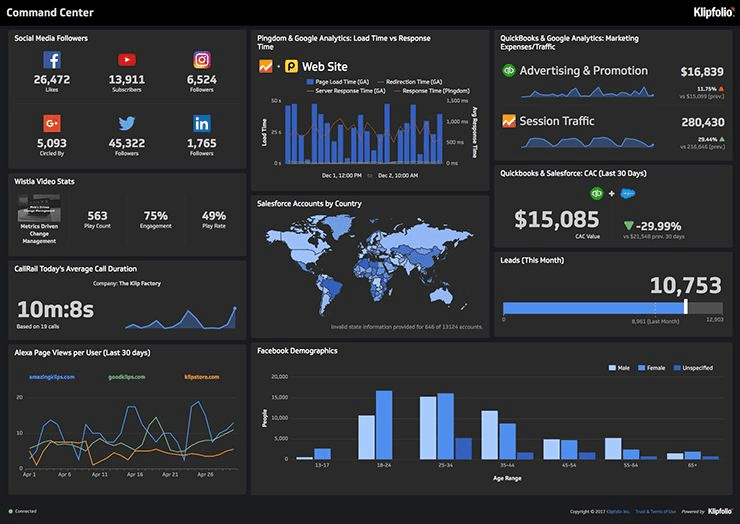
\includegraphics{../figuras/cap07-dashboard-node-red.png}
\caption[Figura 7.3 -- Dashboard Node-RED: painel de supervisão]{Figura 7.3 -- Dashboard Node-RED: painel de supervisão. \textbf{Fonte:} \emph{Node-RED --- Interface de Supervisão} (material do curso), p.~4.}
\end{figure}

O painel foi montado apenas com widgets do \passthrough{\lstinline!node-red-dashboard!}: medidores do tipo \passthrough{\lstinline!gauge!} para
os valores instantâneos, \passthrough{\lstinline!chart!} para as tendências e \passthrough{\lstinline!text!} para os totais. Dois pontos merecem
atenção didática. Primeiro, os blocos de \emph{status} no topo repetem a mesma ideia de \textbf{visão geral}
(nível 1) discutida no Capítulo 11. Segundo, o painel convive com uma imagem ao vivo de câmera no
mesmo quadro --- recurso comum em supervisão de acesso e logística, mas que \textbf{não} deve competir
com as variáveis de processo pela atenção do operador.

\hypertarget{exemplo-de-flow-completo-com-dashboard}{%
\subsection{Exemplo de Flow Completo com Dashboard}\label{exemplo-de-flow-completo-com-dashboard}}

\begin{lstlisting}
[mqtt in] --> [function: payload] --> [gauge: temperatura]
                                  --> [chart: tendencia]
                                  --> [function: alarme]
                                  --> [notification]
[button: resetar] --> [mqtt out: reset]
\end{lstlisting}

\begin{center}\rule{0.5\linewidth}{0.5pt}\end{center}

\hypertarget{integrauxe7uxe3o-com-influxdb-e-grafana}{%
\section{Integração com InfluxDB e Grafana}\label{integrauxe7uxe3o-com-influxdb-e-grafana}}

Para histórico e visualização avançada, o Node-RED integra-se facilmente com InfluxDB:

\hypertarget{instalauxe7uxe3o-1}{%
\subsection{Instalação}\label{instalauxe7uxe3o-1}}

\begin{lstlisting}
node-red-contrib-influxdb
\end{lstlisting}

\hypertarget{node-influxdb-out}{%
\subsection{\texorpdfstring{Node \texttt{influxdb\ out}}{Node influxdb out}}\label{node-influxdb-out}}

Configuração:
- Host: \passthrough{\lstinline!localhost!} (ou IP do servidor InfluxDB)
- Database: \passthrough{\lstinline!industrial\_data!}
- Measurement: \passthrough{\lstinline!temperatura\_reator1!}

O node recebe uma mensagem com \passthrough{\lstinline!msg.payload!} contendo os campos a gravar:

\begin{lstlisting}
// Preparar dados para InfluxDB (formato line protocol)
msg.payload = [
    {
        measurement: "temperatura",
        tags: { equipamento: "reator1", planta: "unidade_A" },
        fields: { valor: msg.payload },
        timestamp: new Date()
    }
];
return msg;
\end{lstlisting}

O \textbf{Grafana} se conecta ao InfluxDB como fonte de dados e exibe dashboards ricos, com alertas e anotações automáticas.

\begin{caixafigura}

\textbf{{[}Figura 7.4 -- Pipeline Node-RED \ensuremath{\rightarrow} InfluxDB \ensuremath{\rightarrow} Grafana{]}}
\emph{Diagrama do pipeline: SCADA/CLP \ensuremath{\rightarrow} Node-RED (flow de coleta e transformação) \ensuremath{\rightarrow} InfluxDB (séries temporais) \ensuremath{\rightarrow} Grafana (dashboard). Screenshot do Grafana mostrando painel com múltiplas variáveis industriais, seletor de período e alerta configurado.}

\end{caixafigura}

\begin{center}\rule{0.5\linewidth}{0.5pt}\end{center}

\hypertarget{node-red-versus-scada-comercial}{%
\section{Node-RED versus SCADA Comercial}\label{node-red-versus-scada-comercial}}

\textbf{Tabela 7.1 -- Comparativo Node-RED \ensuremath{\times} SCADA Comercial}

\begin{longtable}[]{@{}
  >{\raggedright\arraybackslash}p{(\columnwidth - 4\tabcolsep) * \real{0.3333}}
  >{\raggedright\arraybackslash}p{(\columnwidth - 4\tabcolsep) * \real{0.3333}}
  >{\raggedright\arraybackslash}p{(\columnwidth - 4\tabcolsep) * \real{0.3333}}@{}}
\toprule\noalign{}
\begin{minipage}[b]{\linewidth}\raggedright
Critério
\end{minipage} & \begin{minipage}[b]{\linewidth}\raggedright
Node-RED
\end{minipage} & \begin{minipage}[b]{\linewidth}\raggedright
SCADA Comercial (ex.: Ignition, AVEVA)
\end{minipage} \\
\midrule\noalign{}
\endhead
\bottomrule\noalign{}
\endlastfoot
\textbf{Custo} & Gratuito (open-source) & Licença cara (US\$ 5k--500k+) \\
\textbf{Curva de aprendizado} & Baixa & Média a alta \\
\textbf{Sinóticos gráficos} & Limitado (dashboard básico) & Rico: P\&IDs, animações, SVG \\
\textbf{Segurança / acesso} & Básica (plugin) & Controle de acesso robusto, LDAP \\
\textbf{Historização} & Via plugins externos & Nativa, otimizada \\
\textbf{Alarmes} & Manual (flow) & Motor de alarmes dedicado, ISA-18.2 \\
\textbf{Suporte} & Comunidade & Suporte profissional 24/7 \\
\textbf{Certificação} & Não certificado & IEC 62443, FDA 21 CFR Part 11 \\
\textbf{Redundância} & Manual (infraestrutura) & Nativa e testada \\
\textbf{Escalabilidade} & Milhares de tags (com cuidado) & Centenas de milhares de tags \\
\end{longtable}

\textbf{Quando usar Node-RED:}
- Prototipagem e provas de conceito.
- Integrações e glue code entre sistemas.
- Dashboards de monitoramento complementares.
- Projetos educacionais.
- Planta pequena com baixo requisito de disponibilidade.

\textbf{Quando usar SCADA comercial:}
- Infraestruturas críticas (energia, água, óleo e gás).
- Requisitos de certificação regulatória (FDA, ISO, ANEEL).
- Operação 24/7 com SLA de disponibilidade.
- Equipe de operação sem perfil técnico de programação.

O desenho que vem se consolidando na indústria não é ``Node-RED \textbf{ou} SCADA'': é cada um no seu
papel, com o comando e a proteção no CLP e no SCADA, e a integração no Node-RED.

\begin{center}
\IfFileExists{../figuras/capitulo-07-m2.pdf}{%
  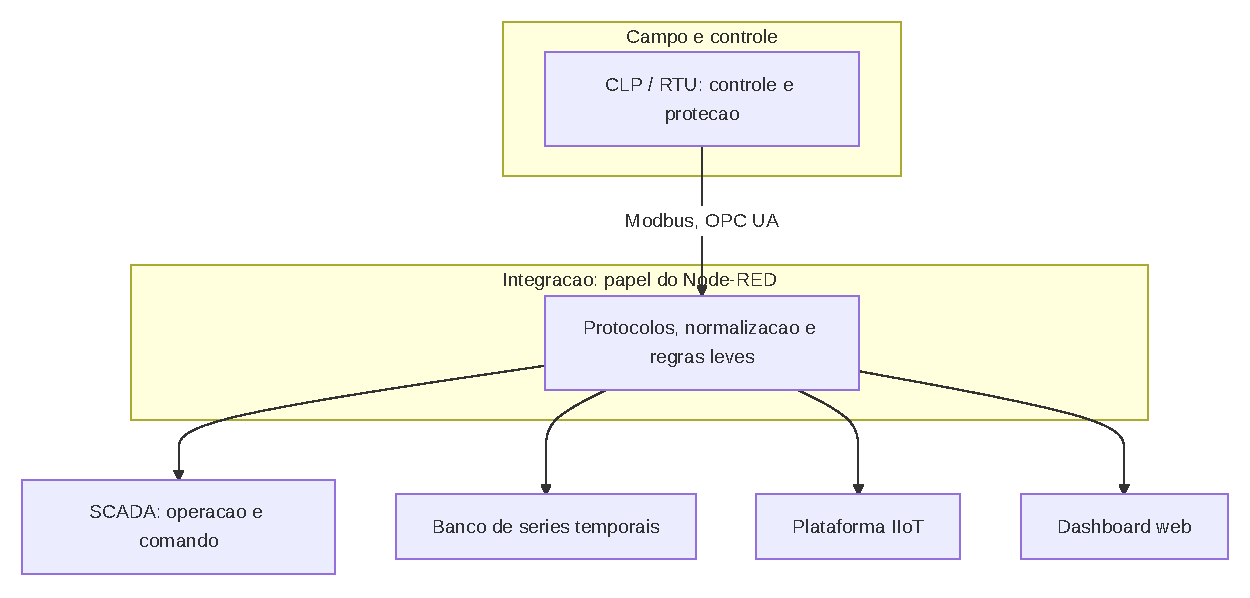
\includegraphics[width=\linewidth,height=0.8\textheight,keepaspectratio]{../figuras/capitulo-07-m2.pdf}%
}{\fbox{\parbox{0.9\linewidth}{\small Diagrama Mermaid ainda não renderizado: capitulo-07-m2. Rode scripts/render-mermaid.sh.}}}
\end{center}

\begin{center}\rule{0.5\linewidth}{0.5pt}\end{center}

\hypertarget{estudo-de-caso-node-red-como-camada-de-integrauxe7uxe3o-em-uma-planta-piloto}{%
\section{\texorpdfstring{Estudo de Caso --- Node-RED como camada de integração em uma planta-piloto}{Estudo de Caso  Node-RED como camada de integração em uma planta-piloto}}\label{estudo-de-caso-node-red-como-camada-de-integrauxe7uxe3o-em-uma-planta-piloto}}

\textbf{Cenário.} Planta-piloto de uma indústria de alimentos, com um CLP de médio porte controlando um
tanque de mistura e temperatura. O CLP não tem OPC UA nem MQTT: expõe Modbus TCP. A equipe de
processo quer acompanhar a curva de temperatura sem esperar pelo projeto corporativo de SCADA,
que está na fila há oito meses.

\textbf{Arranjo montado.} Um microcomputador na rede de controle roda o Node-RED. O fluxo tem três
trechos, cada um com um papel claro:

\begin{enumerate}
\def\labelenumi{\arabic{enumi}.}
\tightlist
\item
  \textbf{Coleta} --- \emph{nodes} \passthrough{\lstinline!modbus-read!} leem os registradores de temperatura e velocidade do
  agitador, em ciclo de 2 s.
\item
  \textbf{Tratamento} --- um \emph{node} \passthrough{\lstinline!function!} converte o inteiro de 16 bits em valor de engenharia
  (escala e \emph{offset} do transmissor), aplica o \emph{deadband} de 0,2 \ensuremath{^\circ}C e marca a qualidade do dado
  quando o CLP não responde.
\item
  \textbf{Distribuição} --- os mesmos dados vão para três destinos: \passthrough{\lstinline!mqtt out!} para o broker, \passthrough{\lstinline!influxdb    out!} para o banco de séries temporais e \passthrough{\lstinline!ui\_gauge!} / \passthrough{\lstinline!ui\_chart!} para o dashboard web.
\end{enumerate}

\begin{lstlisting}
[modbus-read: temperatura]
      |
      v
[function: escala + deadband + qualidade]
      |
      +--> [mqtt out: planta/tanque/temperatura]
      +--> [influxdb out: processo]
      +--> [ui_chart: tendencia de 8 h]
\end{lstlisting}

\textbf{Resultado.} A equipe de processo passou a ter a curva de temperatura no navegador em três dias
de trabalho. Quando o projeto corporativo de SCADA entrou em operação, o mesmo fluxo continuou
rodando ao lado, agora consumindo OPC UA e servindo a plataforma de analytics.

\textbf{Limitações que precisam ser ditas em voz alta.}

\begin{itemize}
\tightlist
\item
  \textbf{Sem redundância.} Se o microcomputador reiniciar, a coleta para; o CLP continua controlando,
  mas o registro tem buraco. Para um piloto é aceitável; para um registro regulatório, não.
\item
  \textbf{Sem trilha de auditoria.} Qualquer pessoa com acesso ao editor altera o fluxo; não há
  controle de versão nem aprovação. Versionar o JSON do fluxo é o mínimo.
\item
  \textbf{Node-RED não substitui o motor de alarmes.} O alarme montado com \passthrough{\lstinline!switch!} + \passthrough{\lstinline!notification!}
  não tem reconhecimento, supressão nem \emph{timestamp} de origem --- os requisitos tratados no
  Capítulo 10 continuam valendo.
\item
  \textbf{Comando não é papel do Node-RED.} Partida de bomba, abertura de válvula e intertravamento
  pertencem ao CLP e ao SCADA.
\end{itemize}

\begin{center}\rule{0.5\linewidth}{0.5pt}\end{center}

\hypertarget{resumo}{%
\section{Resumo}\label{resumo}}

\begin{itemize}
\tightlist
\item
  \textbf{Node-RED} é uma plataforma de programação visual flow-based, open-source, ideal para integrações e supervisão simples.
\item
  Conceitos fundamentais: \textbf{nodes}, \textbf{wires}, \textbf{flows} e \textbf{context}.
\item
  Módulos \passthrough{\lstinline!node-red-contrib-modbus!} e \passthrough{\lstinline!mqtt in/out!} permitem integração com CLPs e brokers MQTT.
\item
  O módulo \passthrough{\lstinline!node-red-dashboard!} gera interfaces web de supervisão sem necessidade de HTML/CSS.
\item
  A integração com \textbf{InfluxDB + Grafana} fornece histórico e visualização de alto nível.
\item
  Node-RED \textbf{complementa} SCADA comercial; raramente o substitui em aplicações críticas.
\end{itemize}

\begin{center}\rule{0.5\linewidth}{0.5pt}\end{center}

\hypertarget{questuxf5es-de-revisuxe3o}{%
\section{Questões de Revisão}\label{questuxf5es-de-revisuxe3o}}

\textbf{Conceituais:}

\begin{enumerate}
\def\labelenumi{\arabic{enumi}.}
\tightlist
\item
  O que é programação \emph{flow-based}? Como ela difere da programação sequencial tradicional?
\item
  Qual é a estrutura de uma mensagem (\passthrough{\lstinline!msg!}) no Node-RED? Quais campos são padrão?
\item
  Cite três vantagens e três limitações do Node-RED como solução supervisória industrial.
\end{enumerate}

\textbf{Práticas:}

\begin{enumerate}
\def\labelenumi{\arabic{enumi}.}
\setcounter{enumi}{3}
\tightlist
\item
  Crie (descreva o flow) para: ler a temperatura de um CLP via Modbus TCP (registrador 40010, float32), exibir em um gauge no dashboard, gerar um alarme no painel se temperatura \textgreater{} 90\ensuremath{^\circ}C e gravar em InfluxDB a cada 5 segundos.
\item
  Como você configuraria o Node-RED para operar com autenticação de usuário e HTTPS? Quais configurações no arquivo \passthrough{\lstinline!settings.js!} seriam necessárias?
\end{enumerate}

\textbf{Desafio:}

\begin{enumerate}
\def\labelenumi{\arabic{enumi}.}
\setcounter{enumi}{5}
\tightlist
\item
  Implemente um flow Node-RED que: (a) subscreva ao tópico MQTT \passthrough{\lstinline!fabrica/+/temperatura!}; (b) calcule a média móvel das últimas 10 leituras; (c) publique a média em \passthrough{\lstinline!fabrica/media/temperatura!}; (d) exiba em um gráfico de tendência no dashboard. Descreva a lógica JavaScript do node \passthrough{\lstinline!function!}.
\end{enumerate}

\begin{center}\rule{0.5\linewidth}{0.5pt}\end{center}

\hypertarget{referuxeancias}{%
\section{Referências}\label{referuxeancias}}

\begin{itemize}
\tightlist
\item
  NODE-RED. \emph{Node-RED Documentation}. Disponível em: \url{nodered.org/docs}.
\item
  OpenJS Foundation. \emph{Node-RED GitHub Repository}. \url{github.com/node-red/node-red}.
\item
  MQTT.ORG. \emph{MQTT Essentials}. Disponível em: mqtt.org.
\item
  INFLUXDATA. \emph{Node-RED InfluxDB Integration}. Disponível em: docs.influxdata.com.
\item
  MATERIAL DE ORIGEM: \emph{Node-Red\_InterfaceDeSupervisão} (material do curso) --- telas do editor e do
  dashboard reproduzidas com crédito.
\end{itemize}
